\documentclass[12pt]{article}
% \usepackage{fullpage}
\usepackage{microtype}
\usepackage{epic}
\usepackage{eepic}
\usepackage{paralist}
\usepackage{graphicx}
\usepackage{algorithm,algorithmic}
\usepackage{tikz}
\usepackage{xcolor,colortbl}
\usepackage{wrapfig}
\usepackage{float}
\usepackage[font=small,labelfont=bf]{caption}


%%%%%%%%%%%%%%%%%%%%%%%%%%%%%%%%%%%%%%%%%%%%%%%%%%%%%%%%%%%%%%%%
% This is FULLPAGE.STY by H.Partl, Version 2 as of 15 Dec 1988.
% Document Style Option to fill the paper just like Plain TeX.

\typeout{Style Option FULLPAGE Version 2 as of 15 Dec 1988}

\topmargin 0pt
\advance \topmargin by -\headheight
\advance \topmargin by -\headsep

\textheight 8.9in

\oddsidemargin 0pt
\evensidemargin \oddsidemargin
\marginparwidth 0.5in

\textwidth 6.5in
%%%%%%%%%%%%%%%%%%%%%%%%%%%%%%%%%%%%%%%%%%%%%%%%%%%%%%%%%%%%%%%%

\pagestyle{empty}
\setlength{\oddsidemargin}{0in}
\setlength{\topmargin}{-0.8in}
\setlength{\textwidth}{6.8in}
\setlength{\textheight}{9.5in}


\def\ind{\hspace*{0.3in}}
\def\gap{0.1in}
\def\bigap{0.25in}
\newcommand{\Xomit}[1]{}

\author{Jonathan Gao}

\linespread{1.15}

\begin{document}
\pagestyle{plain}

\begin{titlepage}
    \begin{center}
        \vspace*{5cm}
        {\huge\textbf{CPU governance and scheduling using machine learning implemented on a Linux kernel}}\\
        \vspace{1.5cm}
        {\large Fall 2020 semester report}
        \vspace{1.5cm}
        
        \textbf{Jonathan Gao}
        \vfill
        \vspace{0.8cm}
        Cornell University\\
        \today
        
    \end{center}
\end{titlepage}

\section*{Introduction}

\ind As an exploratory dive into the Linux kernel, I plan to modify the Linux scheduler to use learned decisions from a machine learning model. At this project's inception, there were many potential options for where a machine learning model may be practical. As an introduction, I will discuss several of those options, the research done in regards to those paths, and the planned route onwards. 

\subsection*{The Scheduler}

\ind The scheduler in an operating system manages the job of ``scheduling'' processes. A operating system deals with numerous processes, all wanting to perform some task using CPU and memory. However, a modern computer may often only have a few cores or processing units, each only capable of running one process at once. Therefore, the operating system must decide which process gets to run on a processor for how long.

Scheduling decisions can be based on a number of parameters. Some simple scheduler implementations include the First In First Out (FIFO) scheduler, where processes get CPU runtime at a first-come-first-served basis. However, this is scheduler is clearly suboptimal, as we care about parameters such as process latency, process deadlines, and overall process throughput. Thus, we have the notion of a CPU quantum, where a process given a CPU quantum will be given a short CPU runtime, say 20ms, before it is taken off and put back onto the process queue.

CPU quanta introduced to the FIFO scheduler becomes the Round Robin scheduler, where the processes get run in FIFO order, and then get enqueued back onto the queue if it does not complete execution within its quantum. The terminology for the notion of a period of execution for a process has been referred to by several names, but has since become the primarily point of focus for modern CPU schedulers.

Scheduling a process is no trivial task, and extensive work has been done to implement an optimal scheduler. Most modern operating systems implement one of the two following schedulers, the Multi-level Feedback Queue scheduler (MLFQ) or the Completely Fair Scheduler (CFS). For example, Windows and macOS use versions of the MLFQ scheduler, whereas Linux has primarily used the CFS scheduler. I considered both of these schedulers for possible machine learning modifications, both of which will be discussed in the following sections.

\subsubsection*{MLFQ schedulers}

\ind Multi-level feedback queue schedulers use several queues rather than the single process queue discussed earlier. The ``multi-level'' queues correspond to different levels of time quanta on the CPU. The highest queue has the shortest quanta on the CPU, with each subsequent queue having longer quanta. With several queues, processes placed onto these queues will run for the time quantum specified by its queue. The number of queues and the range of time quanta will vary, but this structure allows for processes to be classified into groups based on their needs \cite{MultilevelQueue2018}. Using this model, we can prioritize interactive and I/O bound processes by introducting priorities, preemption, and feedback across the queues.

With this model, a process enters the MLFQ scheduler at the top queue with the shortest time quantum. If this process finishes execution within this time quantum, it will terminate and exit the scheduler. Otherwise, if the process relinquishes control of the processor within this time quantum, it will be placed back onto the queue it was dequeued from. However, if this process requires more execution time, it will be preempted at the end of its time quantum and enqueued onto the queue with the next largest time quantum. This process will continue until the process either ends up in a queue optimal for its burst time, the time quantum that it requires before it relinquishes the processor, or ends up in the last queue \cite{MultilevelFeedbackQueue2020,DifferenceMultilevelQueue2020}.

Notice that this design prioritizes short processes that quickly relinquish the processor after execution. However, there are a few concerns with this design. Processes can potentially be ``starved'' from CPU time, where shorter processes constantly come in and prevent those in the lower queues from executing. This can be solved by periodically reinserting lower processes back into the top of the queues. Starvation, along with other concerns such as priority inversion, is one of the disadvantages of using a MLFQ. Much work has been done to mitigate these disadvantages, and the versions in both Windows and macOS likely have such modifications. 

\subsubsection*{Potential routes for the MLFQ scheduler for machine learning}

\ind With the levels of a MLFQ scheduler being a classification problem, I had considered implementing a support vector machine classifier to predict which queue a process will end up in, avoiding the need for feedback and overhead for preemption and moving queues. Rather, processes will be enqueued onto the queue in which the classifier predicts through learned decisions on process metadata. 

Considering that MLFQ schedulers require all processes to ``bubble'' down to their respective queues, a classifier may be able to quickly and efficiently learn which queue a process should be enqueued onto. With a perfect classifier, this can simplify the MLFQ scheduler to a simpler Multi-level queue scheduler, where processes remain on their queues until termination. 

Using support vector machines, the classification of processes can be trained over time using data from a multi-level feedback queue. Once trained, scheduling a process using the SVM will still be O(1) as SVM classifiers simply use a matrix multiplication to perform classification. The classifier can also continously be trained over new data collected from the MLFQ, as the classfier should minimize feedback but will not eliminate it completely.

However, the Linux kernel does not implement a Multi-level Feedback Queue Scheduler, thus any modifications must be done on my implementation of a MLFQ scheduler. This may have been possible, as the real-time \texttt{SCHED\_RR} scheduler offers 99 priority levels with a round robin scheduling policy. A MLFQ scheduler could have been built as a wrapper around this, but was ultimately decided against in preference for routes with the CFS scheduler that will be mentioned.

Several papers surrounding work with machine learning optimizations for MLFQ schedulers has shown some promising results, but seem relatively limited in scope. For example, this implementation of a SVM classifier for a MLFQ \cite{satyanarayanaImprovedProcessScheduling2018} uses only three queues in their own implementation, with some simulation giving questionably improved results. Another paper showed promising results for using reinforcement learning to similarly optimize how feedback in the MLFQ scheduler performs \cite{rinkuReinforcementLearningBased2020}. This paper notes higher CPU utilization across multiple cores as well as lower turnaround and completion time of a batch of processes. While these papers focus around real-time operating systems, I would imagine that standard interactive operating systems will benefit more from machine learning implementations due to greater variety of processes. 

\subsubsection*{The CFS}

\ind The Completely Fair Scheduler aims to be completely fair, as the name suggests, for all processes regardless of the process \cite{DocumentationSchedulerScheddesignCFS}. The underlying mechanism lies in the red-black tree that all processes get inserted to. CFS does not use CPU quanta, but rather tracks the runtime of every process and aims to be divide up CPU time fairly. For example, as from this documentation \cite{DocumentationSchedulerScheddesignCFS}, CFS will schedule two processes such that they both receive 50\% of CPU runtime. The ordered red-black tree maintains a balanced sorted tree of process runtime, where at each scheduler tick the process with the least runtime will be picked. With a bit of granularity to improve cache performance and reduce overhead, the CFS guarantees every process will eventually be able to run.

This scheduler implementation only offers one tunable parameter: the granularity at which a process must overtake the minimum runtime of all processes before another process is selected. Since Linux 2.6, the CFS has remained the default scheduler implementation, though with several changes and improvements since its inception. 

Then, without much to change and tweak in this scheduler, what does machine learning offer for CFS? Despite no tunable parameters for the scheduler itself besides granularity, CFS has features that allow some tweaking of how processes behave relative to one another. 

\subsubsection*{Niceness}

\ind CFS revamps a priority-like value for every process called niceness \cite{InfluenceSchedulingPriority2006}. Process niceness comes from the idea of how ``nice'' a process is to other processes, or how willing they are to give up CPU time for other processes. A process has nice values ranging from -20 to +19, with all processes starting with a default nice value of 0 or otherwise inherited from its parent process. Niceness values indicate how much CPU time a process will consume relative to other processes' niceness. Processes that all have niceness values of 0 will share CPU time equally. However, if two processes have nice values of 0 and +19 respectively, the second process will only take up 5\% of CPU runtime. A curve for niceness to CPU utilization is shown in Figure \ref{fig:niceness}.

\begin{figure}
    \centering
    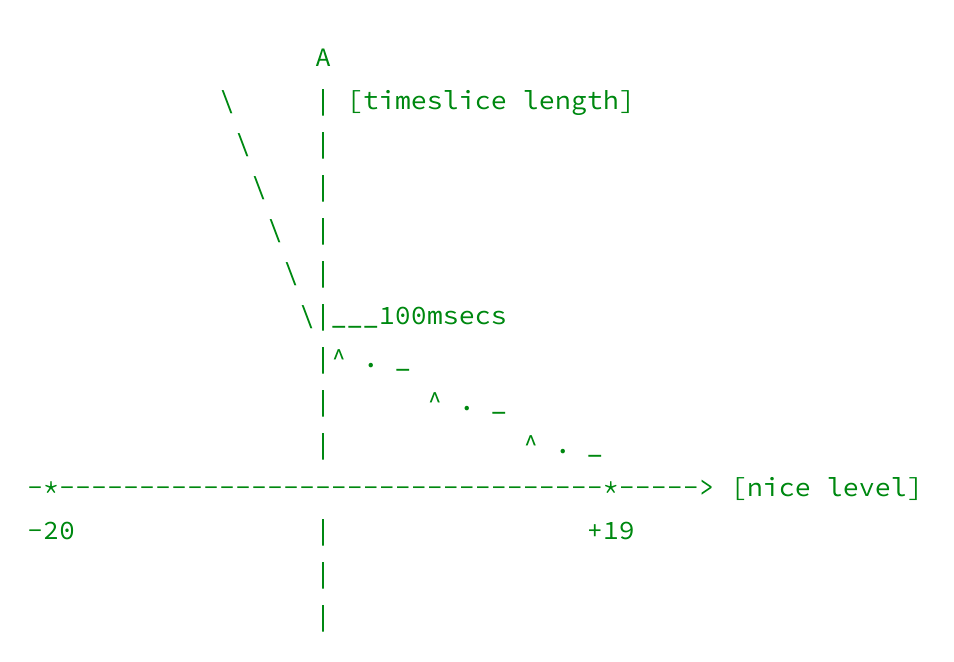
\includegraphics[width=0.9\textwidth]{images/niceness.png}
    \caption{Niceness to CPU utilization, as shown from the CFS scheduler documentation \cite{DocumentationSchedulerSchednicedesign}}
    \label{fig:niceness}
\end{figure}

Nice values for processes can be adjusted, almost like how processes are shifted around the queues in MLFQ, to give more CPU time to certain processes and less to others. Rather, we can use these to improve interactivity and improve response time based on process type. Currently, niceness is not set by any operating system feature, thus is a feature available for users to adjust their process behavior. 

Additionally, there is a grouping feature introduced to the CFS to further improve interactivity \cite{heoControlGroupV22015,ControlGroupsLinux}. Control groups in Linux group processes together, where each group has set assigned resources. Instead, a process nice value only affects CPU runtime within a group. The idea of control groups was introduced to Linux to control the resources of groups of processes, where a cgroup could be defined to limit the CPU utilization, memory usage, and other resources such as network bandwidth. Niceness of a cgroup is implemented through CPU quota and period values. The quota of a cgroup is how much CPU runtime processes within the cgroup get within a period \cite{seltzerUnderstandingCgroups2018}. These are usually defined in microseconds. We see that we can similarly limit a cgroup of processes to consume only a percentage of CPU utilization. Cgroups do get a little more complicated, but ultimately are primarily used for containerization of processes. There are two versions of cgroups infrastructure. v1 and v2 both use the same pseudo filesystem at \texttt{/sys/fs/cgroup/}, but use different structures in mounting controllers. We will be focusing on the cgroups v2 implementation \cite{heoControlGroupV22015}. Cgroups2 has a notion of niceness, or rather CPU weight, that can be defined through the traditional niceness values. By setting a value from -20 to +19 in \texttt{cpu.weight.nice} under the cgroup directory, the cgroup service will set the cpu weights for each group according to the nice values \cite{CPUControllerCgroup2}.

How does containerization of processes improve interactivity? Consider the following example, where we have two processes of equal niceness. One of these processes has is single-threaded, while the other spawns 8 threads. Because Linux treats threads identically to processes, we see that the multithreaded process will end up taking 90\% of CPU utilization. Rather, if we constrain a process and its subprocesses within a cgroup, we maintain interactivity such that threaded processes do not overwhelm the CPU.

\subsubsection*{Autogrouping}

\ind An autogrouping feature was introduced in Linux 2.6, where processes are grouped automatically. From the autogrouping documentation under the \texttt{sched} documentation \cite{SchedLinuxManual}, we see that processes spawned under a new session automatically get placed into its own kernel ``task group.'' Despite the same notion of a task group, the autogrouping feature does not use the existing cgroup infrastructure. Unfortunately, this makes all of the different notions of task grouping very confusing. The autogrouping feature is enabled on some kernels and disabled on others, but can be checked by running \texttt{cat /proc/sys/kernel/sched\_autogroup\_enabled}. Task groups are created on a new session created by \texttt{setdsid()}, where all tasks spawned in this group inherit the group of the parent process. There is also another notion of process groups, where each group has its own group ID used by other syscalls for job control and credential management \cite{CredentialsLinuxManual, troanProcessModelLinux2005}. The autogroup functionality uses the same notion of niceness, where a nice value is applied to the entire group. The nice values are found under the \texttt{/proc/\$PID/autogroup} and can be changed to modify the niceness of the group. 

Users have noted that the inclusion of the autogroup feature essentially nullifies the traditional niceness of processes, as now the \texttt{nice} command only gets reflected in the behavior within an autogroup \cite{nburginWhyNiceLevels2019}. Because of this, the \texttt{nice} and \texttt{renice} commands no longer have their intended effect. 
With both cgroups and autogroups both offering management of CPU runtime, these two features do not overlap. More importantly, cgroup configuration will always override the autogroup configuration.

\subsubsection*{Systemd configuration}

\ind Another service was introduced to the Linux kernel that also offers process grouping functionality. This service, systemd, is an improved init daemon that manages essentially all of the systems background processes and services, offers a software platform for all other programs, and replaces the old init daemon in most Linux kernels today \cite{Systemd2020}. We will focus mainly on the management of processes using the cgroup infrastructure discussed before.

Systemd creates cgroups for every service on startup, but uses the cgroup v1 controllers by default. It can use v2 infrastructure as well, but this requires booting the kernel with a special boot flag \texttt{cgroup\_no\_v1=allows} and \texttt{systemd.unified\_cgroup\_hierarchy=1} \cite{CgroupsArchWiki}. With the cgroups v2 infrastructure, we can set weights on the cgroups created by systemd. In Figure \ref{fig:systemd-cgtop}, we see the output of the \texttt{systemd-cgtop} command, which shows the resource utilization of cgroups in the system. This command shows the output with the hierarchy following the cgroup hierarchy.

\begin{figure}
    \centering
    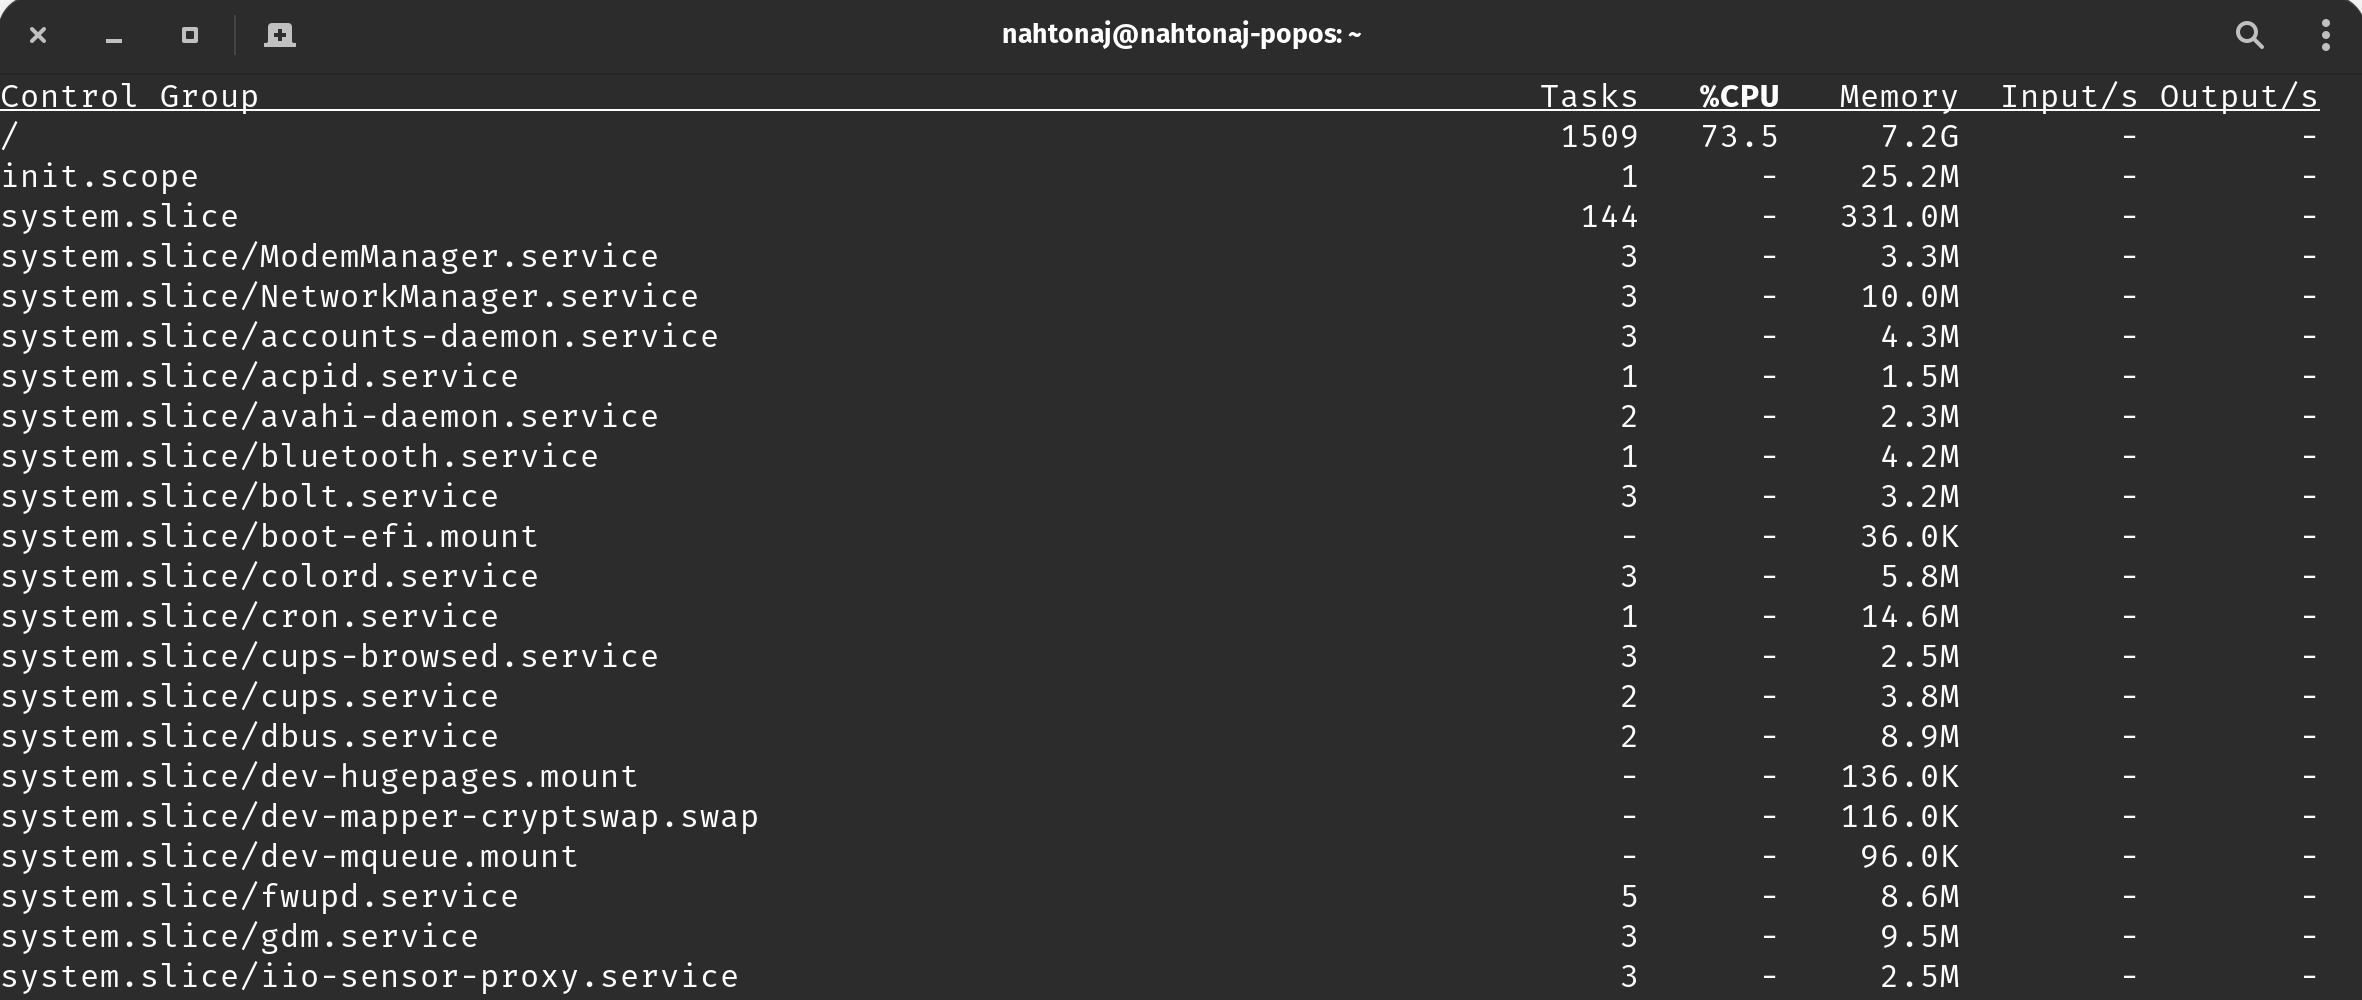
\includegraphics[width=\textwidth]{images/systemd-cgtop.png}
    \caption{\texttt{systemd-cgtop} command output. This shows the cgroups created by \texttt{systemd}, along with CPU and memory utilization. The services shown here are all under the system cgroup, where user services have their own cgroup.}
    \label{fig:systemd-cgtop}
\end{figure}

The systemd service containerizes all services spawned, but does not deal with processes spawned after boot. Rather, processes spawned from new sessions will be grouped by autogrouping. Thus, we notice that process fall into two realms, services run in the background managed by systemd and processes initiated afterwards managed by autogrouping\footnote{This might not be entirely accurate, as my research for systemd and autogrouping is still ongoing. I'm still not quite sure how the autogrouping niceness comes into play with the cgroup parameters. It seems that these two infrastructures are largely separate, so documentation regarding both is fairly limited. Many administrators focused on cgroups infrastructure turn off autogrouping, so this might need a little bit of digging.}. 

\section*{Planned modifications}

\subsubsection*{Using groups instead of processes}

\ind As many have mentioned in forums, blog posts, and articles, the model of completely fair scheduling is not always be the best model. While individual processes can have their CPU timeslice adjusted through niceness, we have already discussed how autogrouping and cgroups have neutered the effectiveness of nice. Rather, the face of multiprocessing has given rise to the dominance of containerization of processes through resource limiting. As of writing this paper, the Linux kernel offers several notions of process grouping, through autogrouping as part of CFS implementation or through cgroups as part of the systemd service. 

Thus, I will focus my modifications on manipulating CPU timeslices of groups of processes. As systemd cgroups mainly contain system services run in the background, I will begin by focusing on the autogrouping functionality of the scheduler. As most background tasks tend to be somewhat less demanding in terms of interactivity, the effects of niceness in autogrouped processes may prove to be more tangible. However, the scope of this work can be easily extended into systemd by reworking the renicing process with the systemd API.

For modifying niceness of autogroups, a daemon can be run modifying the autogroup nice values taken from the \texttt{/proc/} filesystem. Changes made to files here should be validated automatically and nice values should propagate to all processes within the group\footnote{Assuming the autogrouping functionality works how I think it does... The documentation was pretty vague about how parameters get persisted or invoked.}.


\subsubsection*{Regression to determine niceness value for cgroup}

\ind With inspiration from the MLFQ scheduler, I plan to use a regression model or objective function to optimize autogroup niceness over time. The goal is to find the optimal niceness value, or optimal CPU timeslice, over time through feedback. With 40 nice levels, this can essentially be 40 levels where groups will migrate between them based on some feedback. This approach is similar to the one discussed in \cite{rinkuReinforcementLearningBased2020}, where an objective function determined transitions between different queues.

Data about processes can be found in the \texttt{/proc/} filesystem for each process. This includes essentially everything to know about a process, with a few relevant examples including CPU runtime, memory usage, average runtime, context switches, and number of threads.

\subsubsection*{Other notes}

\ind For implementation, I can implement a syscall on a timer that ``renices'' all processes every so often, such that we get dynamic nice values depending on certain factors. This syscall can then be tied to some recurring process, either through a timer interrupt or possibly even just a cron job. This is assuming that renicing processes requires a syscall, as it is possible to simply write with root permissions to the \texttt{/proc/} directory. However, this will require further investigation.

I need to look further into sleeper fairness, which affects I/O bound processes and sleeping processes. This is a concept introduced by the CFS, where the scheduler will try to give sleeping processes a fair share of CPU time right as they wake up.

\section*{Data Collection}

\subsubsection*{Picking workloads}

\ind As many of the references suggest, compiling the Linux kernel is a fairly consistent and reliable workload that can be run with any number of threads. However, because we are not simply measuring a CPU bound workload, we need a variety of workloads to emulate an average user workload. There are a number of benchmark tools available, as seen in this compiled list \cite{LinuxBenchmarkScripts2019}. For interactivity, I found a benchmark that ``emulates the scheduling behavior of interactive tasks and measure[s] their scheduling latency and jitter'' \cite{kolivasCkolivasInterbench2020}. These benchmarks will give me a good comparison of sytem performance before and after my implementation.

Part of my goal is to improve the overall user experience by decreasing latency and improving responsiveness in certain tasks at the cost of reducing performance in others. As mentioned before, not all tasks necessarily deserve a ``fair'' share of CPU runtime. Thus, this will require my machine learning model or objective function to somehow quantify how ``relevant'' or ``interactive'' a process is.

\subsubsection*{Quantifying performance and interactivity}

\ind While the performance of my changes might not be targeted at improving metrics, I will still try to quantify the performance of the system. This includes average turnaround time, process throughput, and average CPU utilization through a variety of workloads.

\subsubsection*{Notes}

\ind Many of the resources below have not been directly referenced or cited. However, all of these resources have contributed to my understanding of the Linux kernel and its functionality. Thus, while the ones cited have direct references to what I mention, the other references have auxiliary information on the topics I discuss.

\nocite{*}
\raggedright
\bibliography{references}
\bibliographystyle{ieeetr}

\end{document}

